\chapter{Cognitivie Biases 1}


Our brains were designed over millions of years by the evolutionary
process. The resulting mind is an amazing and powerful tool, however
not flawless. The human brain has tendencies (or biases) that nudge us
toward bad judgment and poor decisions.

It would be irresponsible to teach you powerful ideas without
also teaching you about the cognitive biases that follow them. There are about 50
that you should know about, but let's start with only a few.

\section{Fundamental Attribution Error}

You tend to attribute
the mistakes of another person to their character, but attribute your
own mistakes to the situation.

Let's say you are at lunch and someone asks you ``Why was Larry late
for class ?''  You are likely to say ``Larry is lazy
and disorganized.''

If someone asks you ``Why were you late for class last week?''  You
are likely to say, ``I don't remember; The class before it must have
run long.''
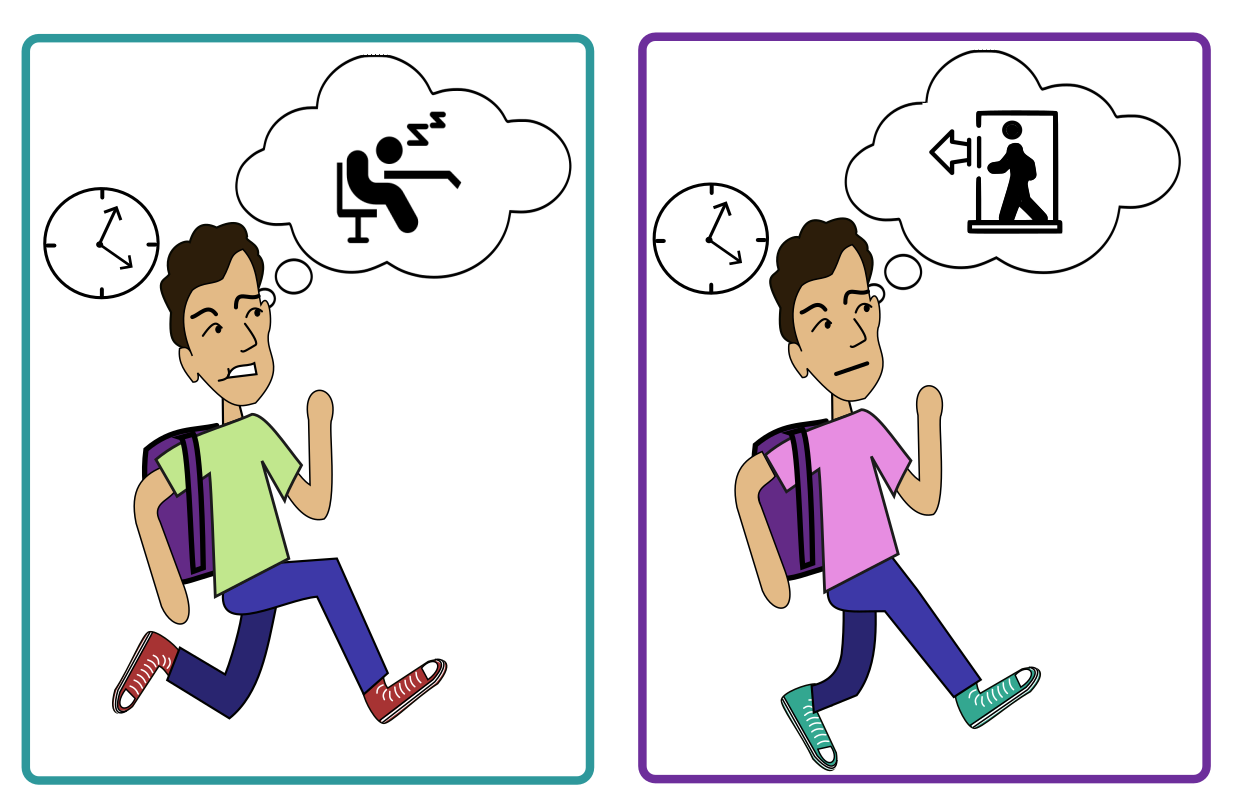
\includegraphics[width=0.8\textwidth]{bias_late.png}

The solution? Cut people some slack. You probably don't know the whole
story, so assume that their character is as strong as yours.

Or maybe you also need to hold yourself to a higher standard? Do you find
yourself frequently rationalizing your bad judgment, lateness, or
rudeness?  This could be an opportunity for you to become a better
person whose character is stronger regardless of the situation.

\section{Self-Serving Bias}

\newterm{Self-serving bias} is when you blame the situation for your
failures, but attribute your successes to your strengths.

For example, when asked ``Why did you lose the match?'' you are likely
to answer ``The referee wasn't fair.''  When you are asked ``Why did
you win the match?'' you are likely to answer ``Because I have been
training for weeks, and I was very focused.''
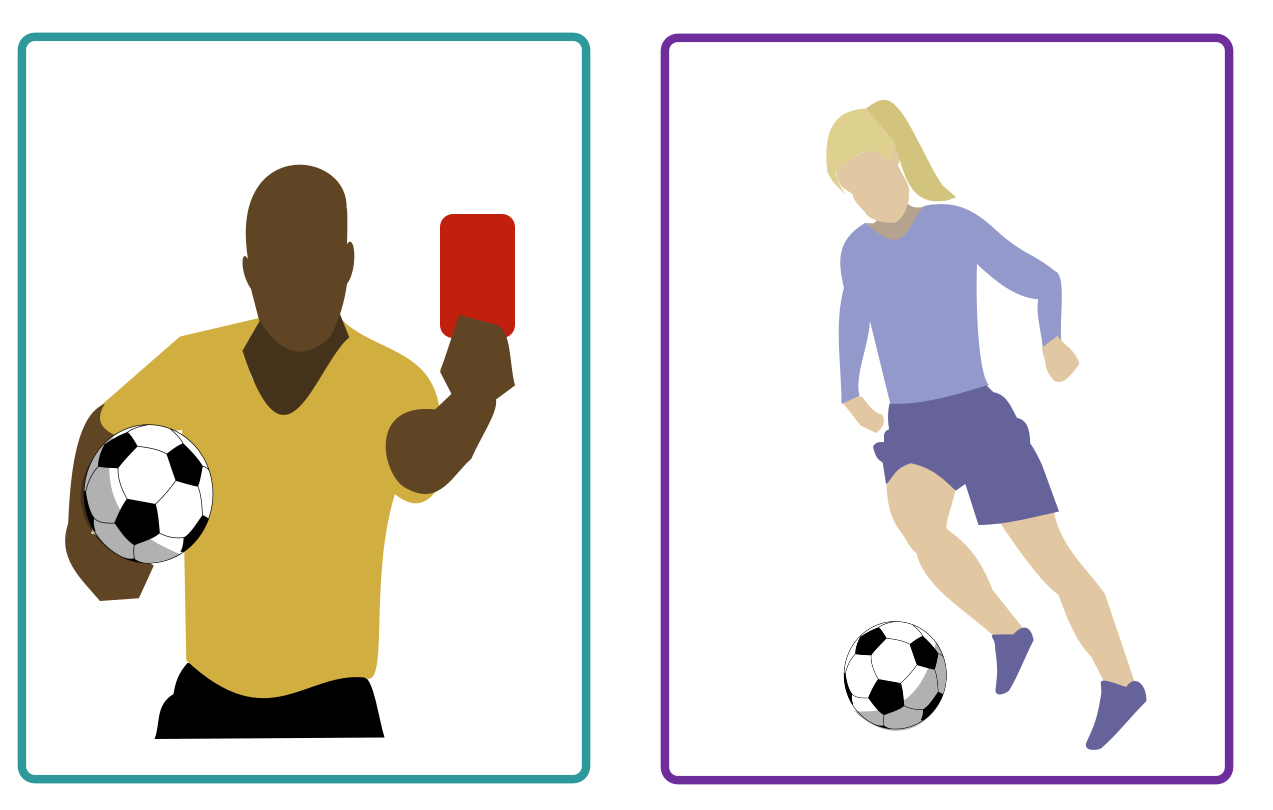
\includegraphics[width=0.8\textwidth]{bias_soccer.png}

This bias tends to make us feel better about ourselves, but it makes it
difficult for us to be objective about our strengths and weaknesses.

\section{In-group favoritism}

\newterm{In-group favoritism}: We tend to favor people who are in
a group with us over people who are not in groups with us.

When asked ``Who is the better goalie, Ted or John?''

If Ted is a Star Trek fan like you, you are likely to think he is also
a good goalie.

As you might imagine, this unconscious tendency is the source of a lot
of subtle discrimination based on race, gender, age, and religion.
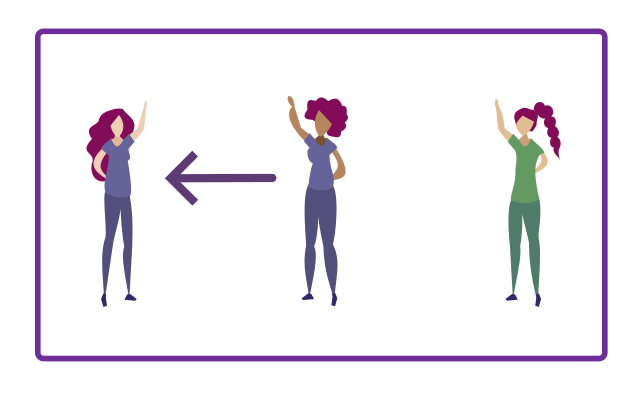
\includegraphics[width=0.8\textwidth]{bias_group.png}

\section{The Bandwagon Effect and Groupthink}

\newterm{The bandwagon effect} is our tendency to believe the same
things that the people around us believe. This is how fads spread so
quickly: one person buys in, and then the people they know have a
strong tencdency to buy in as well.

\newterm{Groupthink} is similar: To create harmony with the
people around us, we go along with things we disagree with.

It takes a lot of perspective to recognize when those around us are
wrong. And it takes even more courage to openly disagree with them.
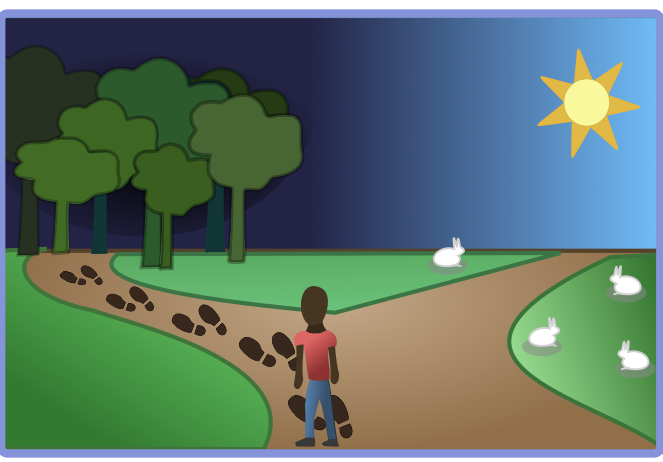
\includegraphics[width=0.8\textwidth]{bias_bandwagon.png}

\section{The Curse of Knowledge}

Once you know something, you tend to assume everyone else knows it too.

This is why teaching is sometimes difficult: a teacher will assume
that everyone in the audience already knows the same things the
teacher knows.

Also, when we learn that a friend doesn't know something that we know,
we are often very surprised. This surprise can sometimes manifest as
hurtful behavior.

When I find a gap in a friend's knowledge, I try to remind myself that
the friend certainly knows many things that I don't. I also try to
imagine how it would feel if they teased me for my ignorance.
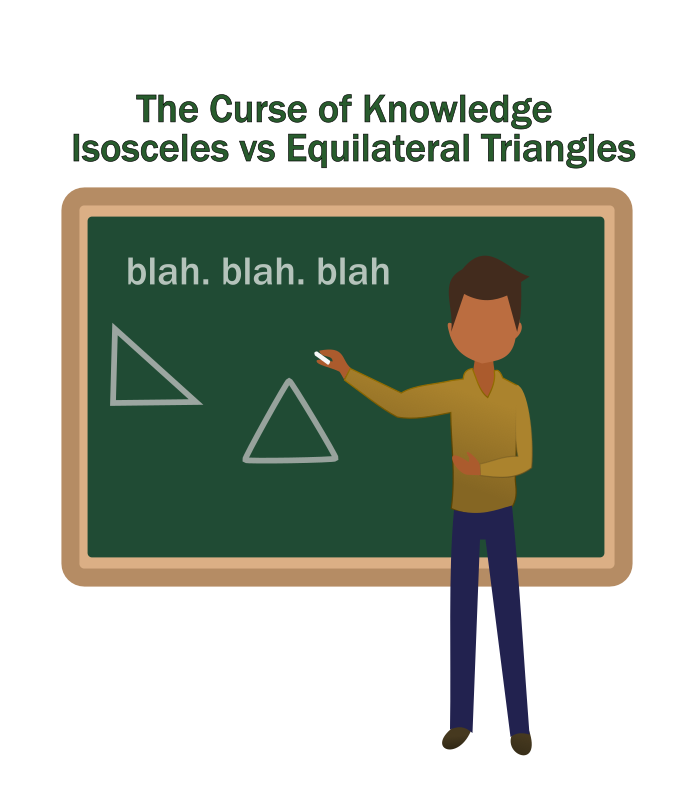
\includegraphics[width=0.8\textwidth]{bias_COK.png}

\section{False Consensus}

We tend to believe that more people agree with us than is actually
the case. For example, if you are a member of a particular religion,
you tend to overestimate the percentage of people in the world who are
members of that religion.

When people vote in elections, they are often surprised when their
preferred candidate loses. ``Everyone, and I mean EVERYONE, voted for
Smith!'' they yell.  ``There must have been a mistake in counting the
votes.''
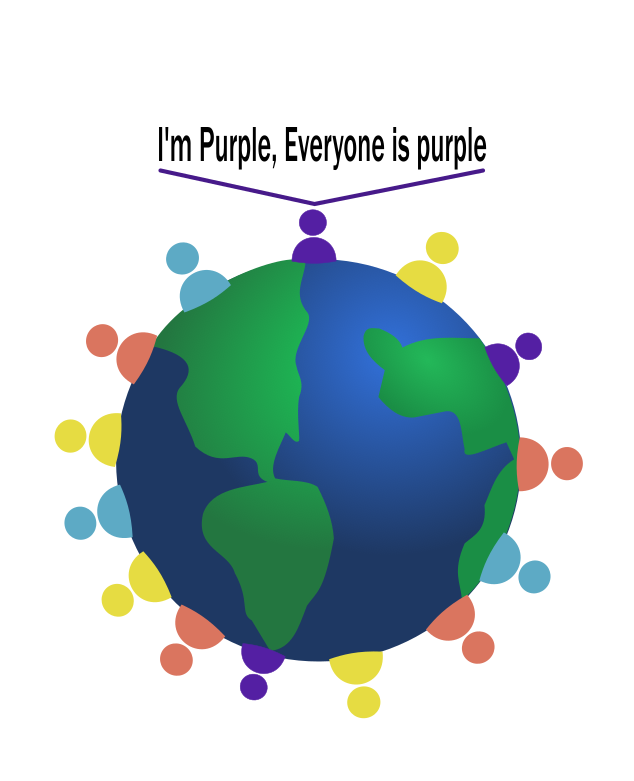
\includegraphics[width=0.8\textwidth]{bias_FC.png}

\section{The Spotlight Effect}

You tend to overestimate how much other people are paying attention to
your behavior and appearance.

Think of six people that you talked to today. Can you even remember what
shoes most of them were wearing? Do you care? Do you think any of them
remember which shoes you wore today?

There is an old saying ``You would worry a lot less about how people
think of you, if you realized how rarely they do.''

\section{The Dunning-Kruger Effect}

The less you know, the more confident you are.

When a person doesn't know all the nuance and context in which a question is
asked, the question seems simple. Thus the person tends to be confident in
their answer. As they learn more about the complexity of the space in
which the question lives, they often realize the answer is not nearly so
obvious.

For example, a lot of people will confidently proclaim ``Taxes are too
high! We need to lower taxes.''  An economist who has studied
government budgets, deficits, history, and monetary policy, might say
something like ``Maybe taxes \emph{are} too high. Or maybe they are
too low. Or maybe we are taxing the wrong things. It is a 
complex question.''

When I am talking with people about a particular topic, I do my best
to defer to the person in the conversation who I think has the most
knowledge in the area. If I disagree with the person, I try to figure
out why our opinions are different.

Similarly, you should assume that any opinion that is voiced, specifically, in an
internet discussion is wildly over-simplified. If you really care
about the subject, read a book by a respected expert. Yes, a whole
book -- there are few interesting topics that can be legitimately
explained in less than 100 pages.
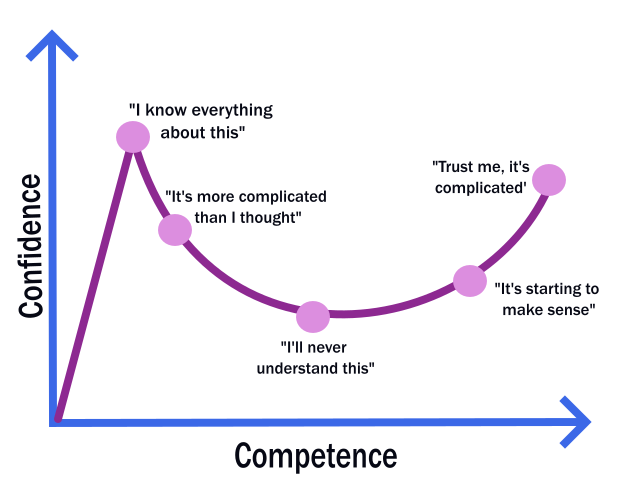
\includegraphics[width=0.8\textwidth]{bias_DK.png}

\section{Confirmation Bias}

You tend to find and remember information that supports
beliefs you already have. You tend to avoid and dismiss information
that contradicts your beliefs.

If you believe that intelligent creatures have visited from other
planets, you will tend to look for data to support your beliefs. When
you find data that shows that it is just too far for any creature to
travel, you will try to find a reason why the data is incorrect.

Confirmation bias is one reason why people don't change their beliefs
more often.

Confirmation bias wrecks many, many studies. The person doing the
study often has a hypothesis that they believe and very much want to
prove true. It is very tempting to discard data that doesn't support
the hypothesis. Or maybe the person throws all the data away and experiments again and again until they get the result they want.

When you design an experiment, you must describe it explicitly before
you start. You must tell someone: ``If the hypothesis I love is
incorrect, the results will look like this.  If the hypothesis I love
is correct, the results will look like that. And if the results look
any other way, I have neither proved nor disproved the hypothesis.''

Once the experiment is underway, you must not change the plan and you
must not discard any data.

This is scientific integrity. You should demand it from yourself, and
you should expect it from others.

\section{Survivorship bias}

You will pay more attention to those that survived a process than
those who failed.

After looking at a lot of old houses, you might say ``In the 1880s,
they built great houses.'' However, you haven't seen the houses that
were built in the 1880s and didn't survive. Which houses tended to
survive for a long time? Only the great houses -- you are
basing your opinion on a very skewed sample.

